\documentclass[titlepage, a4paper]{article}
\usepackage[swedish]{babel}
\usepackage[utf8]{inputenc}
\usepackage{color}

% Sidformat
\usepackage{a4wide}

% Fixa Appendix-titlar
\usepackage[titletoc,title]{appendix}

% Bättre bildtexter
\usepackage[margin=10pt,font=small,labelfont=bf,labelsep=endash]{caption}

% Enkelt kommando som låter mig attgöra-markera text
\newcommand{\todo}[1] {\textbf{\textcolor{red}{#1}}}

%% Headers och Footers
\usepackage{fancyhdr}
\pagestyle{fancy}
\lhead{}
\rhead{\today}
\lfoot{\LIPSkursnamn \\ \LIPSdokumenttyp}
\cfoot{\thepage}
\rfoot{\LIPSprojektgrupp \\ \LIPSprojektnamn}

%% Titelsida
\newcommand{\LIPSTitelsida}{%
{\ }\vspace{45mm}
\begin{center}
  \textbf{\Huge \LIPSdokument}
\end{center}
\begin{center}
  {\Large Redaktör: \LIPSredaktor}
\end{center}
\begin{center}
  {\Large \textbf{Version \LIPSversion}}
\end{center}
\vfill
\begin{center}
  {\large Status}\\[1.5ex]
  \begin{tabular}{|*{3}{p{40mm}|}}
    \hline
    Granskad & \LIPSgranskare & \LIPSgranskatdatum \\
    \hline
    Godkänd & \LIPSgodkannare & \LIPSgodkantdatum \\
    \hline
  \end{tabular}
\end{center}
\newpage
}


% Projektidentitet
\newenvironment{LIPSprojektidentitet}{%
{\ }\vspace{45mm}
\begin{center}
  {\Large PROJEKTIDENTITET}\\[0.5ex]
  {\small
  \LIPSartaltermin, \LIPSprojektgrupp\\
  Linköpings Tekniska Högskola, MAI
  }
\end{center}
\begin{center}
  {\normalsize Gruppdeltagare}\\
  \begin{tabular}{|l|l|p{25mm}|l|}
    \hline
    \textbf{Namn} & \textbf{Ansvar} & \textbf{Telefon} & \textbf{E-post} \\
    \hline
}%
{%
    \hline
  \end{tabular}
\end{center}
\begin{center}
  {\small
    \textbf{E-postlista för hela gruppen}: \LIPSgruppadress\\
    \textbf{Hemsida}: \LIPSgrupphemsida\\[1ex]
    \textbf{Kund}: \LIPSkund\\
    \textbf{Kontaktperson hos kund}: \LIPSkundkontakt\\
    \textbf{Kursansvarig}: \LIPSkursansvarig\\
    \textbf{Handledare}: \LIPShandledare\\
  }
\end{center}
\newpage
}
\newcommand{\LIPSgruppmedlem}[4]{\hline {#1} & {#2} & {#3} & {#4} \\}

%% Dokumenthistorik
\newenvironment{LIPSdokumenthistorik}{%
\begin{center}
  Dokumenthistorik\\[1ex]
  %\begin{small}
    \begin{tabular}{|l|l|p{60mm}|l|l|}
      \hline
      \textbf{Version} & \textbf{Datum} & \textbf{Utförda förändringar} & \textbf{Utförda av} & \textbf{Granskad} \\
      }%
    {%
			\hline
    \end{tabular}
  %\end{small}
\end{center}
}

\newcommand{\LIPSversionsinfo}[5]{\hline {#1} & {#2} & {#3} & {#4} & {#5} \\}

% Kravlistor
\newenvironment{LIPSkravlista}{
	\center
		\tabularx{\textwidth}{| p{1.2cm} | p{1.9cm} | X | c |}
			\hline
			\textbf{Krav} & \textbf{Förändring} & \textbf{Beskrivning} & \textbf{Prioritet} \\\hline
}
{
		\endtabularx
	\endcenter
}

\newcounter{LIPSkravnummer}
\addtocounter{LIPSkravnummer}{1}
\newcommand{\LIPSkrav}[4][Krav \arabic{LIPSkravnummer}]{{#1} & {#2} & {#3} & {#4} \stepcounter{LIPSkravnummer}\\\hline}	% Importera generella layout-strukturer

% Information nödvändig för generella layout-strukturer
\newcommand{\LIPSredaktor}{Pål Kastman}
\newcommand{\LIPSversion}{0.1}
\newcommand{\LIPSdokument}{Projektplan}
\newcommand{\LIPSdokumenttyp}{Projektplan}
\newcommand{\LIPSgranskatdatum}{}
\newcommand{\LIPSgranskare}{}
\newcommand{\LIPSgodkannare}{}
\newcommand{\LIPSgodkantdatum}{}
\newcommand{\LIPSkursnamn}{TSEA29}
\newcommand{\LIPSprojektnamn}{Lagerrobot}
\newcommand{\LIPSprojektgrupp}{Grupp 2}
%\newcommand{\LIPSgruppadress}{}
\newcommand{\LIPSartaltermin}{HT1, 2014}
\newcommand{\LIPSgrupphemsida}{http://github.com/ultralaserdeluxe/gloria}
\newcommand{\LIPSkund}{Tomas Svensson}
\newcommand{\LIPSkundkontakt}{Tomas Svensson}
\newcommand{\LIPSkursansvarig}{Tomas Svensson}
\newcommand{\LIPShandledare}{Peter Johansson}

% Dokument-specifika paket
\usepackage{tabularx}
\usepackage{pdfpages}
\usepackage{tikz}
\usetikzlibrary{shapes, arrows}

\pagenumbering{roman}


\DeclareGraphicsRule{.2.pdf}{pdf}{*}{}

\begin{document}

\LIPSTitelsida

\begin{LIPSprojektidentitet}
\LIPSgruppmedlem{Pål Kastman}{Projektledare}{0703896295}{palka285@student.liu.se}
\LIPSgruppmedlem{Hannes Snögren}{Dokumentansvarig}{0706265064}{hansn314@student.liu.se}
\LIPSgruppmedlem{Alexander Yngve}{Hårdvaruansvarig}{0762749762}{aleyn573@student.liu.se}
\LIPSgruppmedlem{Martin Söderén}{Mjukvaruansvarig}{0708163241}{marso329@student.liu.se}
\LIPSgruppmedlem{Daniel Wassing}{Leveransansvarig}{0767741110}{danwa223@student.liu.se}
\LIPSgruppmedlem{Dennis Ljung}{Testansvarig}{0708568148}{denlj069@student.liu.se}
\end{LIPSprojektidentitet}

\newpage
\tableofcontents	%Innehållsförteckning	
%\listoffigures
%\listoftables

\newpage

\begin{LIPSdokumenthistorik}
\LIPSversionsinfo{0.1}{}{Första utkast}{}{}
\end{LIPSdokumenthistorik}

\newpage
\pagenumbering{arabic}	%Påbörja sidnumrering

% Inledning, översikt osv

\section{Beställare}


\section{Översiktlig beskrivning av projektet}


\subsection{Syfte och mål}
Målet med projektet är att konstruera ett system som autonomt ska kunna röra sig i ett lager. Denna måste uppfylla kravspecifikationen som har tagits fram tillsammans med beställaren. Från en dator skall systemet kunna styras att plocka upp paket. Syftet med projektet är att gruppens medlemmar skall lära sig och få erfarenhet att jobba efter en projektmodell samt ge praktiska kunskaper och erfarenheter när det gäller att jobba med mikroprocessorer, digitala system och elektronikkonstruktion. När projektet är klart ska roboten kunna navigera autonomt längs en bana som är specifierad i banspecifikationen. 
Under projektets gång så ska alla gruppmedlemmar arbeta på ett professionellt sätt och arbeta metodiskt. 

\subsection{Leveranser}

\begin{table}[h]
  \centering
    \begin{tabularx}{\textwidth}{| X | l | l | X | l |}
      \hline
      \textbf{Leverans} & \textbf{Ansvarig} & \textbf{Godkänns av} & \textbf{Beskrivning} & \textbf{Färdig} \\
      \hline

      {Projektplan, tidsplan och systemskiss} & {Daniel} & {} & {Första version av projektplan, tidsplan och systemskiss} & {2014-09-26} \\
            \hline
      {Projektplan, tidsplan och systemskiss} & {Daniel} & {} & {Slutgiltig version av projektplan, tidsplan och systemskiss} & {2014-10-02} \\
      \hline
      {Designspecifikation} & {Daniel} & {} & {Designspecifikation skall vara inlämnad} & {2014-11-04} \\
      \hline
      {Tidsrapport} & {Daniel} & {} & {Tidsrapport 1 skall vara inlämad} & {2014-11-03} \\
      \hline
      {Designspecifikation} & {Daniel} & {} & {Designspecifikation skall vara godkänd} & {2014-11-07} \\
      \hline
      {Tidsrapport} & {Daniel} & {} & {Tidsrapport 2 skall vara inlämad 2014-11-10} & {2014-11-10} \\
      \hline
      {Tidsrapport} & {Daniel} & {} & {Tidsrapport 3 skall vara inlämad} & {2014-11-17} \\
      \hline
      {Tidsrapport} & {Daniel} & {} & {Tidsrapport 4 skall vara inlämad} & {2014-11-24} \\
      \hline
      {Tidsrapport} & {Daniel} & {} & {Tidsrapport 5 skall vara inlämad} & {2014-12-01} \\
      \hline
      {Tidsrapport} & {Daniel} & {} & {Tidsrapport 6 skall vara inlämad} & {2014-12-08} \\
      \hline
      {Tidsrapport} & {Daniel} & {} & {Tidsrapport 7 skall vara inlämad} & {2014-12-15} \\
      \hline
      {Efterstudie} & {Daniel} & {} & {Efterstudie skall vara inlämnad} & {2014-12-19} \\
      \hline
      {Utrustning} & {Daniel} & {} & {Utrustning skall vara inlämnad} & {2014-12-19} \\
      \hline
      {Slutleverans} & {Daniel} & {} & {Roboten skall levereras senast vecka 51} & {2014-12-19} \\
      \hline

    \end{tabularx}
  \caption{Dokumentation} \label{dokumentation:tabell}
\end{table}


\subsection{Begränsningar}

Projektet är begränsat till att uppfylla de krav som angetts i kravspecifikationen. De krav i kravspecifikationen som angetts med annan prioritet än 1 kommer endast att genomföras i mån av tid. Det finns även begränsningar på hur många timmar som kan läggas på projektet. Efter det att projektplanen har blivit godkänd får endast 960 arbetstimmar läggas på projektet. Det finns även en mjuk begränsning på vilka komponenter som finns tillgängliga. Dock så finns möjlighet att köpa in komponenter om det finns ett behov utav dem och de inte är alltför dyra.


\section{Fasplan}
Projektet består av tre faser, före, under och efter.

\subsection{Före projektstart}
Innan projektstart skall kravspecifikation, projektplan, tidsplan och en systemskiss skrivas.

\subsection{Under projektet}
Under projektets gång skall systemet specificeras i en designspecifikation och konstrueras därefter. Det skall även skrivas teknisk dokumentation och användarhanledning för systemet.

\subsection{Efter projektet}
Efter beslutspunkt 5 anses projektet avklarat. Därefter skall systemet levereras tillsammans med teknisk dokumentation och användarhandledning. Systemet skall acceptanstestas av kunden. Efterstudie och slutrapport skall ske efter leverans.

\section{Organisationsplan för hela projektet}

\subsection{Organisationplan per fas}
\todo{Har vi olika grupperingar/organisation beroende på fas? Roller. Rita!}

\subsection{Villkor för samarbete inom projektgruppen}
\todo{Skriv gruppkontrakt}

\subsection{Ansvarsområden}
Varje gruppmedlem är huvudansvarig för olika delar av arbetet enligt tabell \todo{tabellref}.

\begin{table}[h]
  \centering
    \begin{tabularx}{\textwidth}{| l | l | X | l | l | l |}
      \hline
      \textbf{Titel} & \textbf{Ansvarsområde} & \textbf{Vem} \\
      \hline
      {Projektledare} & {} & {} \\\hline
      {} & {} & {} \\\hline
      {} & {} & {} \\\hline
      {} & {} & {} \\\hline
      {} & {} & {} \\\hline
      {} & {} & {} \\\hline
    \end{tabularx}
  \caption{Dokumentation} \label{dokumentation:tabell}
\end{table}


\subsubsection{Roller}
Projektledare Pål
  Huvudsaklig kontaktperson för gruppen. Sköter kontakt med beställare/handledare, sammankallar möten, ordförande i gruppmöten, ansvarig för att alla leveranser sker i rätt tid, ansvarig för att tids-/statusrapporter skrivs och lämnas i tid, ansvarig för att arbetet fortskrider enligt tidsplanen.
Dokument  Hannes
  Ansvarig för att alla dokument skrivs och ser snygga ut. 
Mjukvaruansvarig  Martin
  Huvudsakligen ansvarig för Beagleboarden och programvaran på PC.
Hårdvaruansvarig  Alexander
  Ansvarig för att all hårdvara är rätt, bra virad och fungerar korrekt.
Testansvarig  Dennis
  Ansvarig för att alla delsystem testas ingående för att se till att allt fungerar som tänkt. Ansvarig för att systemet som helhet testas.
Leveransansvarig  Daniel
  Ansvarig för att vi har en bra stämning i gruppen.

\section{Dokumentplan}
Dokumentation listad i tabell \ref{dokumentation:tabell} skall utföras.

\begin{table}[h]
	\centering
		\begin{tabularx}{\textwidth}{| p{22mm} | l | X | p{25mm} | X | l |}
			\hline
			\textbf{Dokument} & \textbf{Ansvarig} & \textbf{Godkänns av} & \textbf{Syfte} & \textbf{Distribue-
  ras till} & \textbf{Färdig datum} \\\hline

			{Systemskiss} & {Daniel} & {Tomas} & {Underlag för Designspecen} & {Gruppen och Tomas} & {2014-10-02} \\\hline
    		{Tidsplan} & {Daniel} & {Tomas}& {Hjälpmedel under projektet} & {Gruppen och Tomas} & {2014-10-02} \\\hline
			{Projektplan} & {Daniel} & {Tomas} & {Hjälpmedel för hur projektet ska utföras} & {Gruppen och Tomas} & {2014-10-02} \\\hline
			{Tidsrapporter} & {Daniel} & {Tomas} & {För att kunna se så alla bidrar} & {Gruppen och Tomas} & {Varje måndag} \\\hline
			{Uppdaterad tidsplan} & {Daniel} & {Tomas} & {Se hur projektet ligger till} & {Gruppen och Tomas} & {Varje måndag} \\\hline
			{Statusrapport för projektet} & {Daniel} & {Tomas} & {Se hur projektet ligger till} & {Gruppen och Tomas} & {Vid begäran} \\\hline
			{Designspec} & {Daniel} & {Peter} & {Underlag för konstruktionen} & {Gruppen och Tomas} & {2014-11-07} \\\hline
            {Teknisk
			dokumentation} & {Daniel} & {Tomas} & {Dokumentera de tekniska lösningarna} & {Gruppen och Tomas} & {2014-12-12} \\\hline
            {Användar-
			handledning} & {Daniel} & {Delges Tomas} & {Manual för användarna} & {Gruppen och Tomas} & {2014-12-12} \\\hline
			{Efterstudie
			dokument} & {Daniel} & {Tomas}& {Reflektera vad som skulle gjorts annorlunda} & {Gruppen och Tomas} & {2014-12-19} \\\hline
		\end{tabularx}
	\caption{Dokumentation.} \label{dokumentation:tabell}
\end{table}


% \section{Utvecklingsmetodik}


\section{Utbildningsplan}

\subsection{Egen utbildning}
Varje gruppmedlem är själv ansvarig för att ta till sig kunskap nödvändig för att kunna utföra sin del av projektet. En referensgrupp finns tillgänglig för kortare utbildning inom specifika områden. En labb kommer genomföras i syfte att utbilda samtliga gruppmedlemmar i användning av logikanalysator. 

\section{Rapporteringsplan}
Rapporter kommer att användas för att ge beställaren en bild av hur projektet fortlöper och om tidsplanen följs. Projektledaren är ansvarig för att dessa rapporter skrivs och levereras till beställaren enligt överrenskommelse.

\subsection{Tidsrapport}
Varje vecka skall en tidsrapport levereras till beställaren. Tidsrapporten ska innehålla vad som har gjorts under veckan och tidsåtgången för detta. Tidsrapporten används främst för att korrigera tidsplanen allteftersom projektet fortlöper.

\subsection{Statusrapport}
På begäran av beställaren skall en statusrapport leveraras. Statusrapporten skall innehålla vilka aktiviteter gruppen jobbar på just nu, vilka aktiviteter som har genomförts och vilka aktiviteter gruppen kommer att göra i nästa skede.


\section{Mötesplan}

Projektledaren sammankallar till projektmöte. Målet är att ha två möten i veckan. Med det första mötet för veckan avses att stämma av hur gruppen ligger till och om några oförutsedda problem har uppstått. Detta möte förväntas inte ta längre tid än en halv timme. I slutet av varje vecka hålls ett möte för att utvärdera och sammanställa veckans arbetsinsatser samt planera efterföljande veckas arbete. Beslut om nödvändiga förändringar i tidsplanen tas av projektledaren i slutet av varje vecka. Detta möte beräknas därför ta mer tid. \\
Projektmöten hålls efter en av två mötesmallar (Se Bilaga \ref{ap:motesmall}) beroende på vilken typ av möte det är. Mötestyp 1 är menat för kortare möte mitt i veckan för att fånga upp problem så tidigt som möjligt. Mötestyp 2 är menat för något längre möte i slutet av arbetsveckan för att summera den gågna veckan och planera efterföljande arbetsvecka.


\section{Resursplan}

\subsection{Personer}
Projektgruppen består av medlemmar enligt tabell \ref{projektplan:resursplan-personer}
\begin{table}[h]
	\centering
		\begin{tabularx}{\textwidth}{| l | l | X | l | l | l |}
			\hline
			\textbf{Namn} & \textbf{Ansvar} & \textbf{E-post} \\
			\hline
			{Pål Kastman} & {Projektledare} & {palka285@student.liu.se} \\\hline
			{Daniel Wassing} & {Leveransansvarig} & {danwa223@student.liu.se} \\\hline
			{Hannes Snögren} & {Dokumentansvarig} & {hansn314@student.liu.se} \\\hline
			{Martin Söderén} & {Mjukvaruansvarig} & {marso329@student.liu.se} \\\hline
			{Alexander Yngve} & {Hårdvaruansvarig} & {aleyn573@student.liu.se} \\\hline
			{Dennis Ljung} & {Testansvarig} & {denlj069@student.liu.se} \\\hline
		\end{tabularx}
	\caption{Medlemmar i projektgruppen} \label{projektplan:resursplan-personer}
\end{table}

\subsection{Material}
Material nödvändig för projektet kommer att förses av beställaren. Om något saknas under projektets gång kontaktar projektledaren beställaren för att undersöka möjligheter att införskaffa detta.

\subsection{Lokaler}
Projektgruppen kommer ha tillgång till Muxen på campus Valla för att konstruera hårdvaran för roboten. Där kommer gruppen ha tillgång till en eller två arbetsplatser. Arbetet kommer försökas delas upp på ett sådant sätt att inte alla gruppmedlemmar behöver vistas vid arbetsstationerna samtidigt. Viss utveckling av framförallt mjukvara kommer vara möjligt att utföra enskilt hemifrån. \\
Möten kommer hållas antingen i det konferensrum som finns tillgängligt i Muxen eller i annan lokal som finns tillgäng på universitetet.

\subsection{Ekonomi}
Projektet har en övre tidsgräns på 960 arbetstimmar efter beslutspunkt 2. Dessa redovisas veckovis till beställaren.

\section{Milstolpar}

\begin{LIPSmilstolpar}
\LIPSmilstolpe{1}{Milstolpe 1: Fungerande kommunikation mellan huvud-, styr- och sensorenhet}{deadline(datum)}
\LIPSmilstolpe{2}{Läs data (driftinfo, sensorvärden) på PC}{}
\LIPSmilstolpe{3}{Robotens samtliga motorer och servon kan styras från PC}{}
\LIPSmilstolpe{4}{Roboten kan följa en linje autonomt}{}
\LIPSmilstolpe{5}{Robotens arm har full funktionalitet}{}
\LIPSmilstolpe{6}{Roboten kan stanna på plockstationer och detektera paket}{}
\LIPSmilstolpe{7}{Roboten är tävlingsklar}{}
\end{LIPSmilstolpar}

%\section{Aktiviteter}

\begin{LIPSaktivitetslista}
	\LIPSaktivitet{1}{Implementation av protokoll mellan huvud- och styrenheten}{}{16}
	\LIPSaktivitet{2}{Koppla ihop huvud- och styrenheten}{}{4}
	\LIPSaktivitet{3}{Implementera buss mellan huvud- och sensorenheten}{}{16}
	\LIPSaktivitet{4}{Koppla ihop huvud- och sensorenheten}{}{4}
	\LIPSaktivitet{5}{Sätta upp utvecklingsmiljö för AVR}{}{8}
	\LIPSaktivitet{6}{Installera mjukvara på huvud (OS, Python, drivare)}{}{10}
	\LIPSaktivitet{7}{Python-modul på PC för att skicka/ta emot data från huvudenheten}{}{16}
\end{LIPSaktivitetslista}
\begin{LIPSaktivitetslista}
	\LIPSaktivitet{8}{Koppla in linjesensorer på sensorenheten}{}{10}
	\LIPSaktivitet{9}{Koppla in IR-sensor på sensorenheten}{}{2}
	\LIPSaktivitet{10}{Koppla in motorer och styrenheten}{}{2}
	\LIPSaktivitet{11}{Koppla in servon på styrenheten}{}{2}
	\LIPSaktivitet{12}{Upprätta BT förbindelse mellan huvudenheten och PC}{6}{10}
	\LIPSaktivitet{13}{Sätta upp utvecklingsmiljö för BeagleBoard (wifi)}{6}{4}
	\LIPSaktivitet{14}{Skriva UI för PC}{7}{20}
	\LIPSaktivitet{15}{Implementera och testa muxning för linjesensor}{8}{8}
	\LIPSaktivitet{16}{Implementera styrning av motorer}{10}{8}
	\LIPSaktivitet{17}{Implementera styrning av servon}{11}{20}
	\LIPSaktivitet{18}{Testa och felsöka buss mellan huvud- och styrenheten}{1,2,13}{16}
	\LIPSaktivitet{19}{Testa och felsöka buss mellan huvud- och sensorenheten}{3,4,13}{16}
	\LIPSaktivitet{24}{Implementera styrlogik}{13}{40}
	\LIPSaktivitet{25}{Implementera läsning av sensorer}{15,9}{16}
	\LIPSaktivitet{26}{Mäta respons från motorer och servon}{16,17}{8}
	\LIPSaktivitet{27}{Implementera tolkning och utförande av kommandon från PC på huvudenheten}{14,19}{12}
	\LIPSaktivitet{28}{Tolka IR-sensordata}{25}{8}
	\LIPSaktivitet{29}{Implementera kalibreringsfunktion}{37}{20}
	\LIPSaktivitet{30}{Implementera tolkning och utförande av kommandon från huvudenheten på sensorenheten}{19,25}{16}
	\LIPSaktivitet{31}{Testa styra servon från styrenheten}{26}{8}
	\LIPSaktivitet{32}{Testa styra motorer från styrenheten}{26}{8}
	\LIPSaktivitet{33}{Testa styra servon från huvudenheten}{18,31}{8}
	\LIPSaktivitet{34}{Testa styra motorer från huvudenheten}{18,32}{8}
	\LIPSaktivitet{35}{Implementera läsning av sensordata på huvudenheten}{19,30}{8}
	\LIPSaktivitet{37}{Skriva testprogram för linjesensor styrenhet}{25}{8}
	\LIPSaktivitet{38}{Implementera och testa X,Y,Z till servovinkel, konvertering}{31}{32}
	\LIPSaktivitet{39}{Implementera och testa gränser för armen}{31}{24}
	\LIPSaktivitet{40}{Implementera smoothing-funktion för servon och motorer}{32}{16}
	\LIPSaktivitet{41}{Implementera paketnersättningsfunktion}{33}{16}
	\LIPSaktivitet{42}{Implementera fjärrstyrning från PC}{27,33,34,35}{16}
	\LIPSaktivitet{43}{Implementera och testa detektion av stoppmarkering}{35,37}{16}
	\LIPSaktivitet{44}{Implementera och testa detektion av paket}{35,36}{16}
	\LIPSaktivitet{45}{Implementera och testa detektion av stationer}{35,37}{16}
	\LIPSaktivitet{46}{Implementera regleringsalgoritm (linjeföljare)}{34,37}{40}
	\LIPSaktivitet{47}{Testa styrlogik}{43,44,45,46}{40}
	\LIPSaktivitet{48}{Möten}{}{72}
	\LIPSaktivitet{49}{Dokumentation: Teknisk Dokumentation}{}{32}
	\LIPSaktivitet{50}{Dokumentation: Tidsrapport}{}{10}
	\LIPSaktivitet{51}{Dokumentation: Användarhandledning}{}{8}
	\LIPSaktivitet{52}{Dokumentation: Efterstudie}{}{8}
	\LIPSaktivitet{53}{Presentation + PP}{}{32}
	\LIPSaktivitet{54}{Tejpa testbanor}{}{3}
	\LIPSaktivitet{55}{Dokumentation: Designspecifikation}{}{100}
	\LIPSaktivitet{56}{Buffertid}{}{103}
\end{LIPSaktivitetslista}


\section{Tidplan}

\todo{Se Bilaga Tidsplan}

\section{Förändringsplan}

I första hand skall förseningar hanteras internt i gruppen genom att justera tidsplanen. Om en försening är så stor att den riskerar att försena en leverans skall projektledaren ta kontakt med beställaren för att diskutera möjliga lösningar. Omförhandlingar av kravspecifikation och leveransdatum skall undvikas.

\section{Kvalitetsplan}

\subsection{Granskningar}
Projektledaren är ansvarig för att tidsplan, scheman och presentation är korrekta och håller hög kvalitet. Varje gruppmedlem granskar sin egen kod. Dokumentansvarig ser över att koden är välkommenterad och välstrukturerad innan inlämning.

\subsection{Testplan}
I första hand skall varje gruppmedlem se till att det han eller hon jobbar på är väl implementerat och fungerar korrekt. Testansvariga verifierar att alla funktioner hos alla delsystem och hela systemet fungerar som planerat.


% \section{Prioriteringar}

\section{Projektavslut}

Projektet avslutas när roboten är acceptanstestad, levererad och både teknisk dokumentation och användarhandledning blivit leverarade. Resultatet av projektet skall efter projektets slut sammafattas i en muntlig presentation. Erfarenheter sammanfattas i en efterstudie.


%\section{Referenser}



\newpage
\begin{appendices}

% Bilagor

\section{Mötesmallar} \label{ap:motesmall}
Följande två dokument är mallar avsedda för projektmöten. 

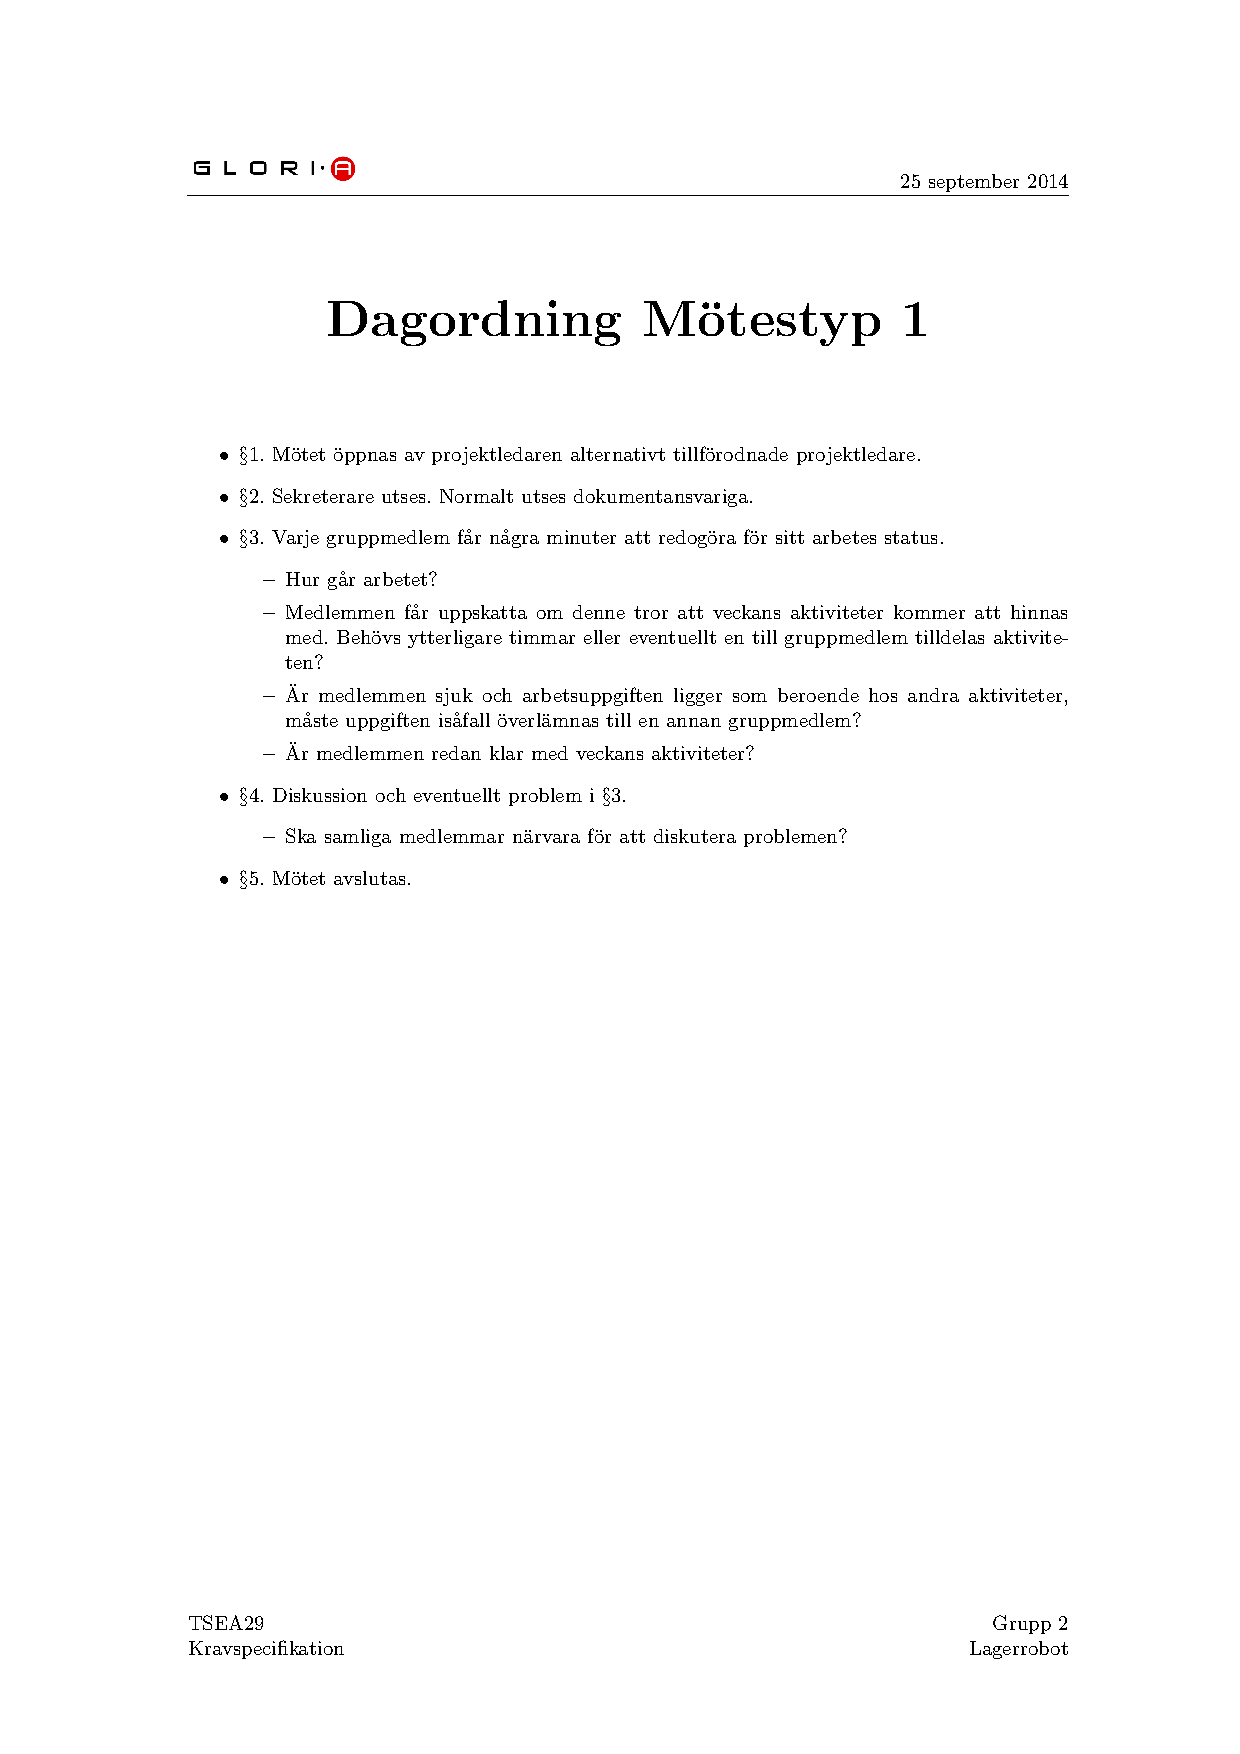
\includepdf[pages=-]{../motesprotokoll/motesmall1.pdf}

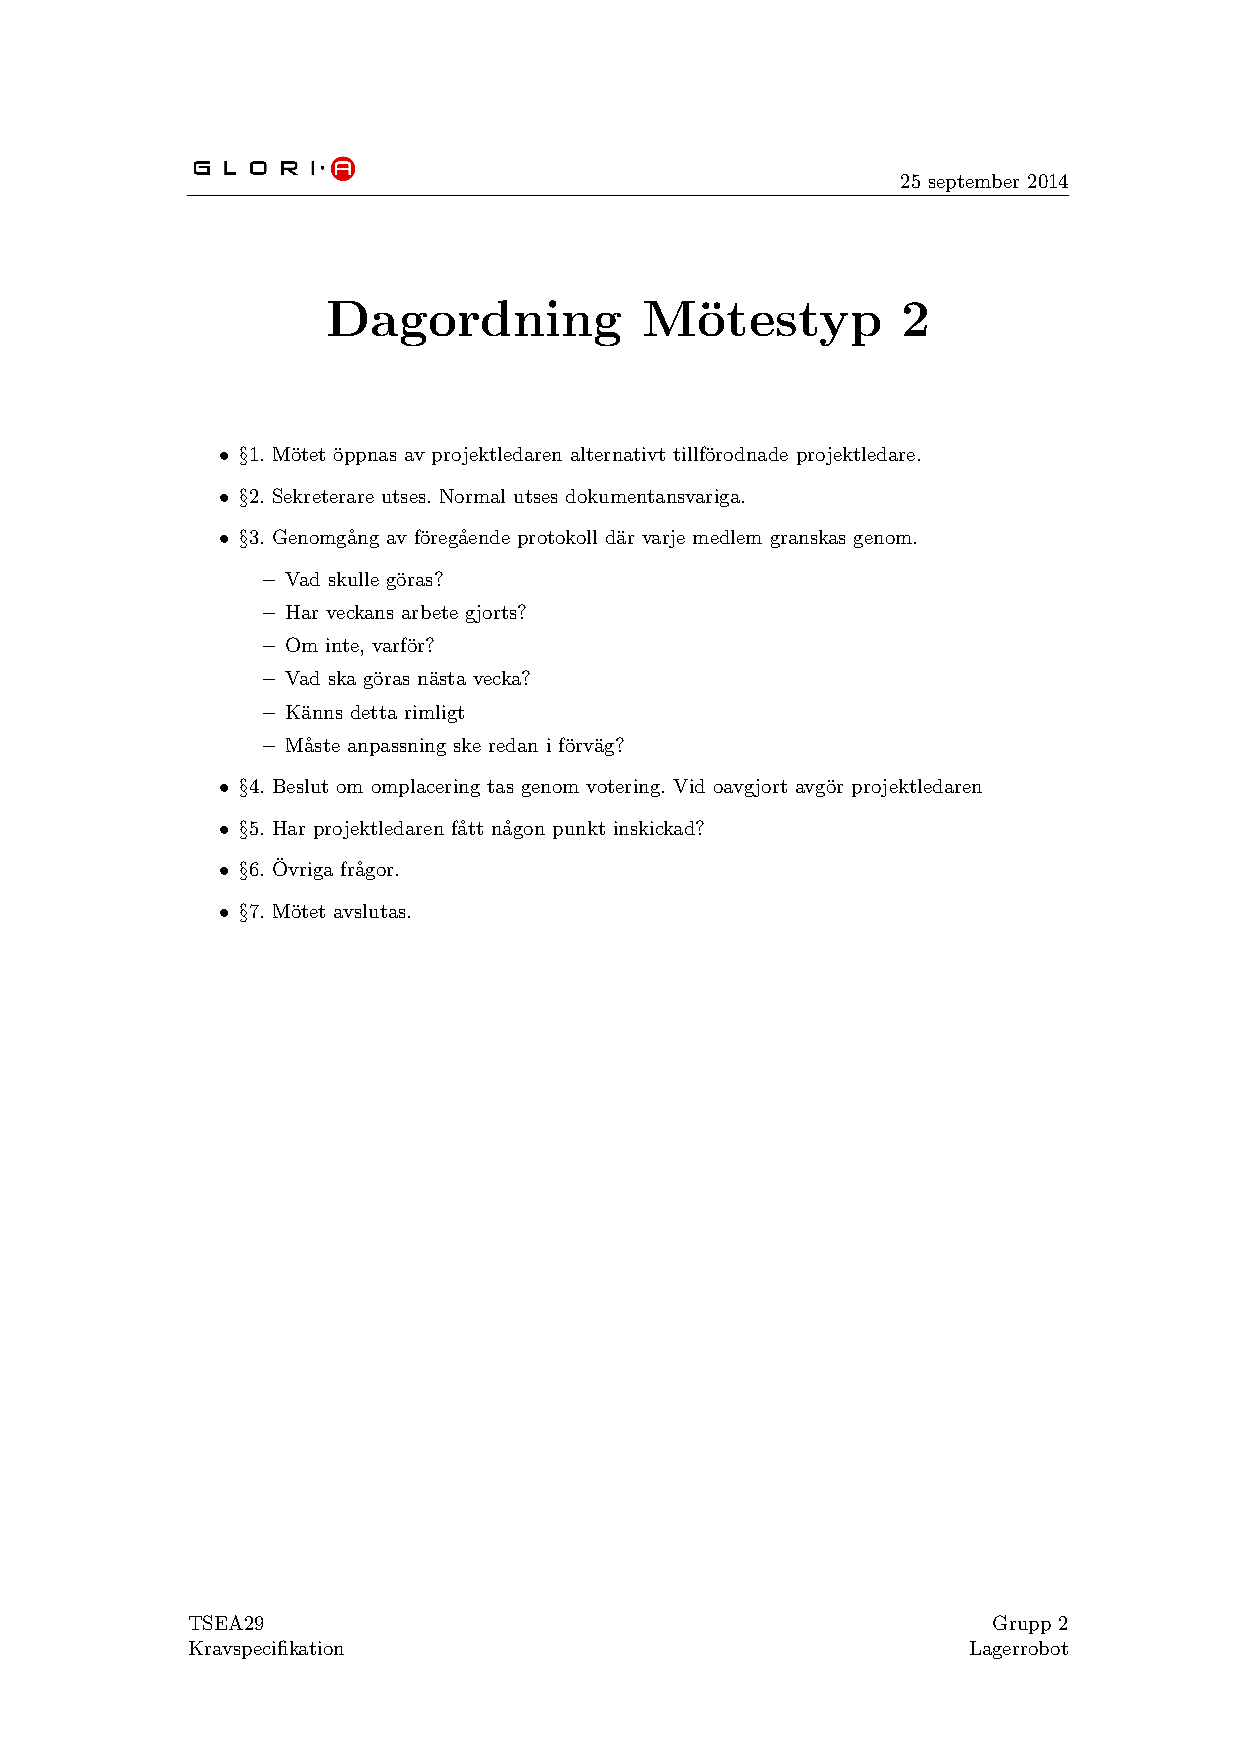
\includepdf[pages=-]{../motesprotokoll/motesmall2.pdf}


\newpage
\section{Tidsplan}
\center
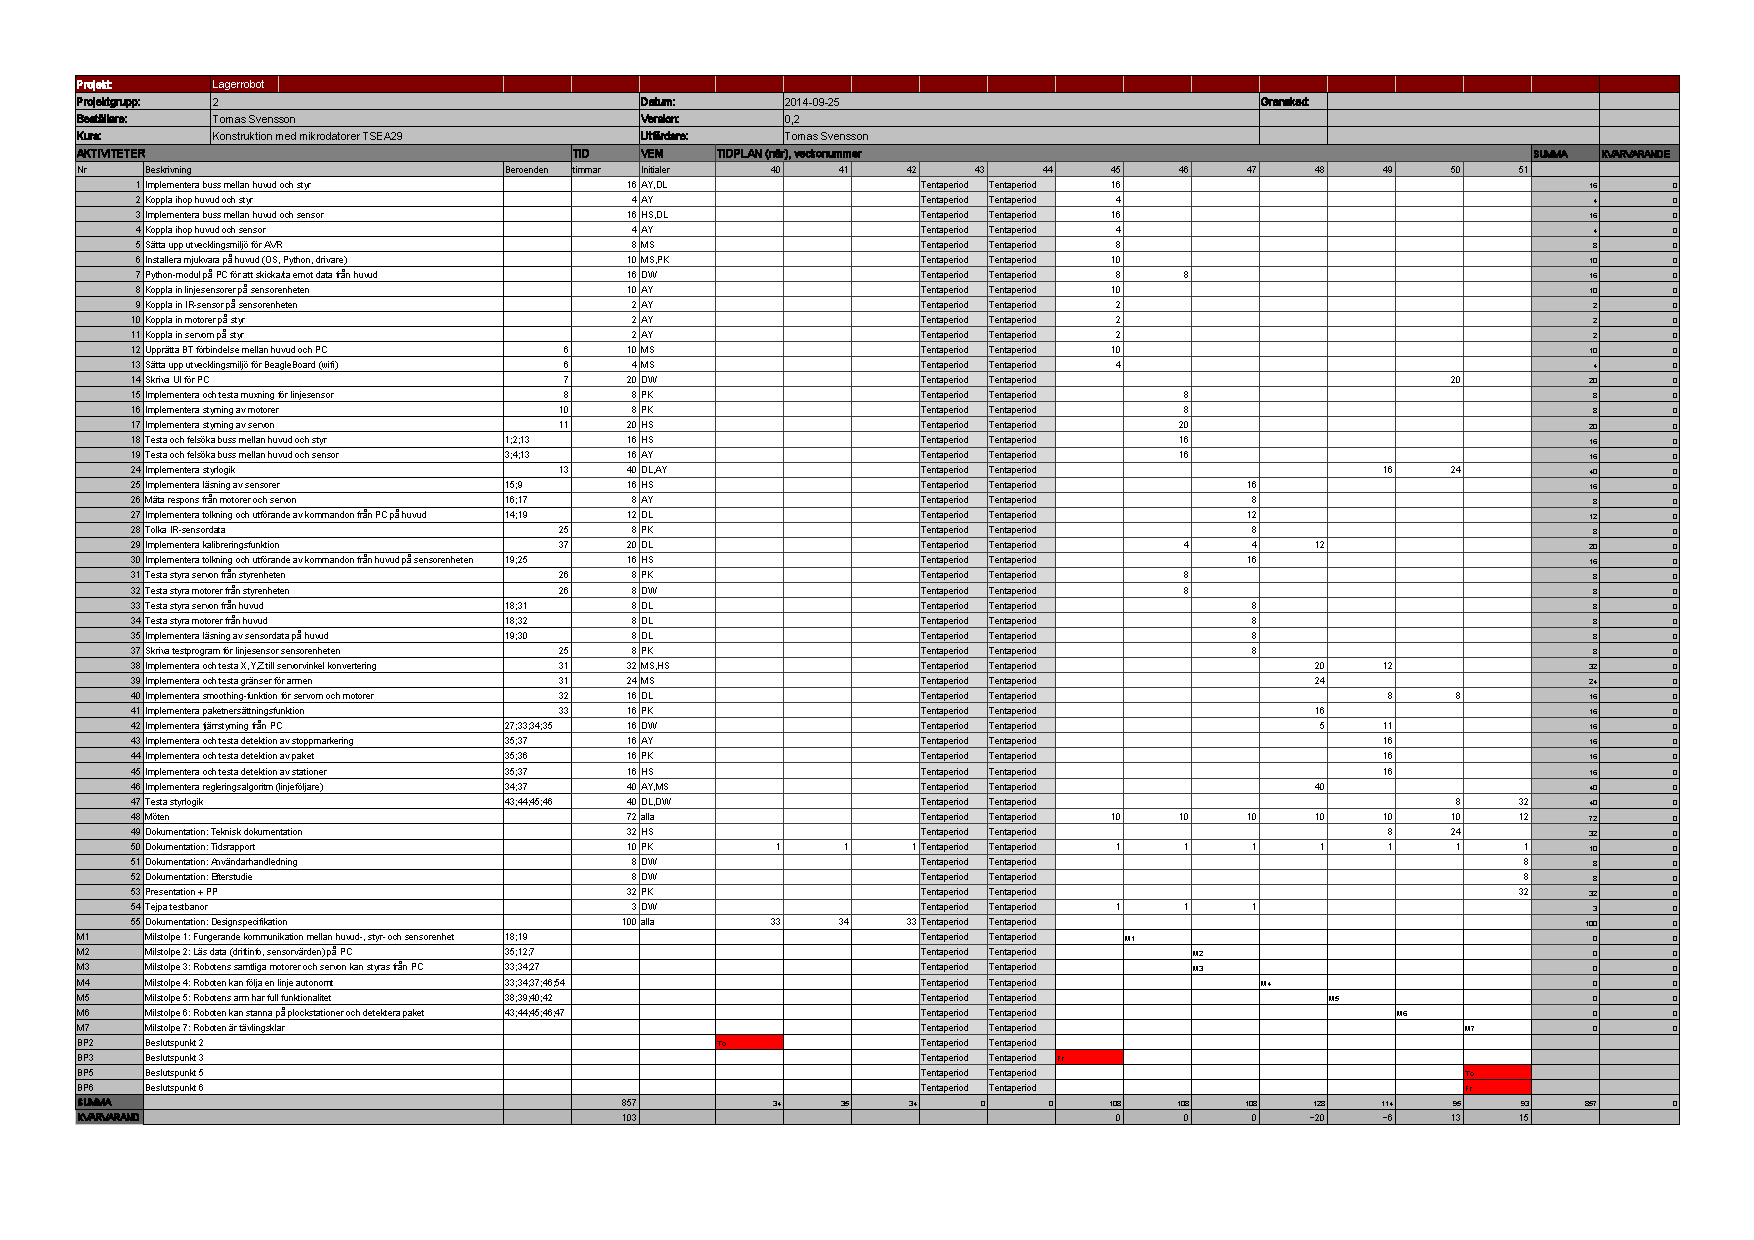
\includegraphics[angle=90, scale=0.7]{../tidsplan/tidsplan_v0.2.pdf}


\end{appendices}


\end{document}
